\svnid{$Id$}
\chapter[AniA and NorB Expression in \Nm{}]{Further Work - AniA and NorB Expression in \Nm{}}
\label{chap:expression}
The expression of AniA and NorB has not been mentioned in this work thus far as it adds a further level of complication to an already complex model. The data shown in the previous chapters shows that it seems to be possible to model, with reasonable accuracy, many of the facets of respiration without the need for modifying the levels of expression of the respiratory enzymes. However regulation of expression systems \textit{do} exist in the respiratory system and it would be an oversight to omit them from discussion here.

Unfortunately due to time constraints it was not possible to fully investigate expression in this respiratory system, however the following was theorised as a potential method for including expression of AniA and NorB in the model.

It is posited that expression of AniA and NorB could be modelled by treating them as being expressed using Michaelis-Menten kinetics. This being the case, the rate of change of the two enzymes in the system can be expressed as differential equations in the following manner:

\begin{eqnarray*}
\frac{d[A]}{dt} & = & \left(R\left(1 - \frac{[O_2] + k_{10}[NO]}{[O_2] + k_{10}[NO] + k_{11}}\right) - S\left(1 - \frac{[NO]}{[NO] + k_{13}}\right)\right) - k_8[A] \nonumber \\ \\
\frac{d[B]}{dt} & = & T \left(\frac{[NO]}{[NO] + k_{15}}\right) - k_{16}[B]
\end{eqnarray*}
The parameters required for NorB expression can be explained simply: $T$ is equivalent to the $V_{max}$ of enzyme expression and $k_{15}$ is equivalent to the $K_M$. $k_{16}$ is included to model the degradation rate of the enzyme. The expression rate of NorB is dependent solely on the concentration of NO present.

AniA expression is more complicated to model as it is not only repressed by oxygen, but activated \textit{and} repressed by NO. The NO activation is modelled by $S$ and $k_{13}$ which correspond to the $V_{max}$ and $K_M$ of the activation respectively. This ensures that AniA isn't expressed when NO is too low. The repression of activation by oxygen and NO is modelled by $R$,$k_{10}$ and $k_{11}$ which represent the $V_{max}$, ``NO inhibition scale factor'', and $K_M$ of the repression respectively. The ``NO inhibition scale factor'' effectively sets the cut-off concentration of NO at which it starts repressing AniA expression. As with NorB expression, $k_8$ here represents the degradation rate of AniA.

The first part of the AniA equation models the regulation by FNR, and the second part in addition to the NorB equation models the regulation by NsrR. As detailed in Chapter \ref{chap:intro}, NsrR is a repressor of both AniA and NsrR, and FNR (Fumarate and nitrite reductase regulator) is an activator of AniA. Nitric Oxide inhibits the NsrR protein leading to an increase in expression of both NorB and AniA since the repression by NsrR is no longer present. Higher concentrations of Nitric Oxide cause FNR to be inhibited which effectively represses AniA. High concentrations of Oxygen also cause inhibition of FNR meaning that AniA isn't expressed until low concentrations of Oxygen are present.

These two new differential equations could easily be incorporated into the model to complement the original 9 equations. There are two datasets which could potentially be used to populate these new parameters. The first is from \citet{Heurlier2008} which details levels of expression in response to regulation by Nitric Oxide (produced by Spearmine NONOate). This is shown in Figure \ref{fig:expression1}.
\begin{figure}[tbp]
 \centering
 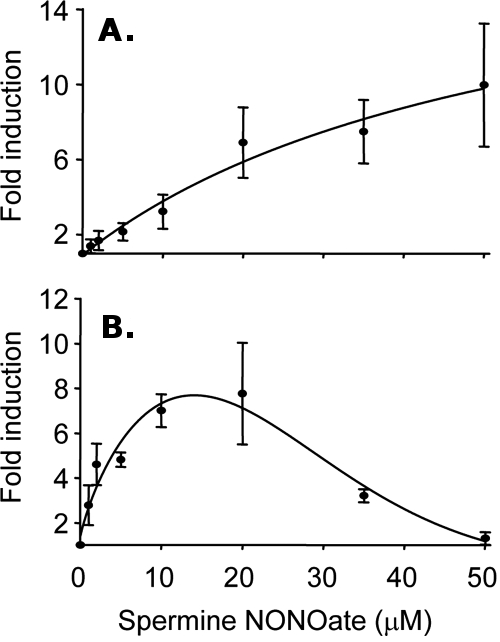
\includegraphics[height=10cm]{./08-expression/data/zjb0070877000001.png}
 % zjb0070877000001.png: 500x642 pixel, 72dpi, 17.64x22.65 cm, bb=0 0 500 642
 \caption[Effect of Nitric Oxide on NsrR and FNR Dependent Gene Expression]{{\bf Effect of Nitric Oxide on NsrR and FNR Dependent Gene Expression}. Expression of (A) NorB and (B) AniA in wild-type \Nsm{}. Figure adapted from \citet{Heurlier2008}.
 \label{fig:expression1}}
\end{figure}
The second is from \citet{Rock2005} which details the effect on Oxygen reduction and Nitric Oxide creation and reduction during microaerobic respiration, and this is shown in Figure \ref{fig:expression}.
\begin{figure}[tbp]
 \centering
 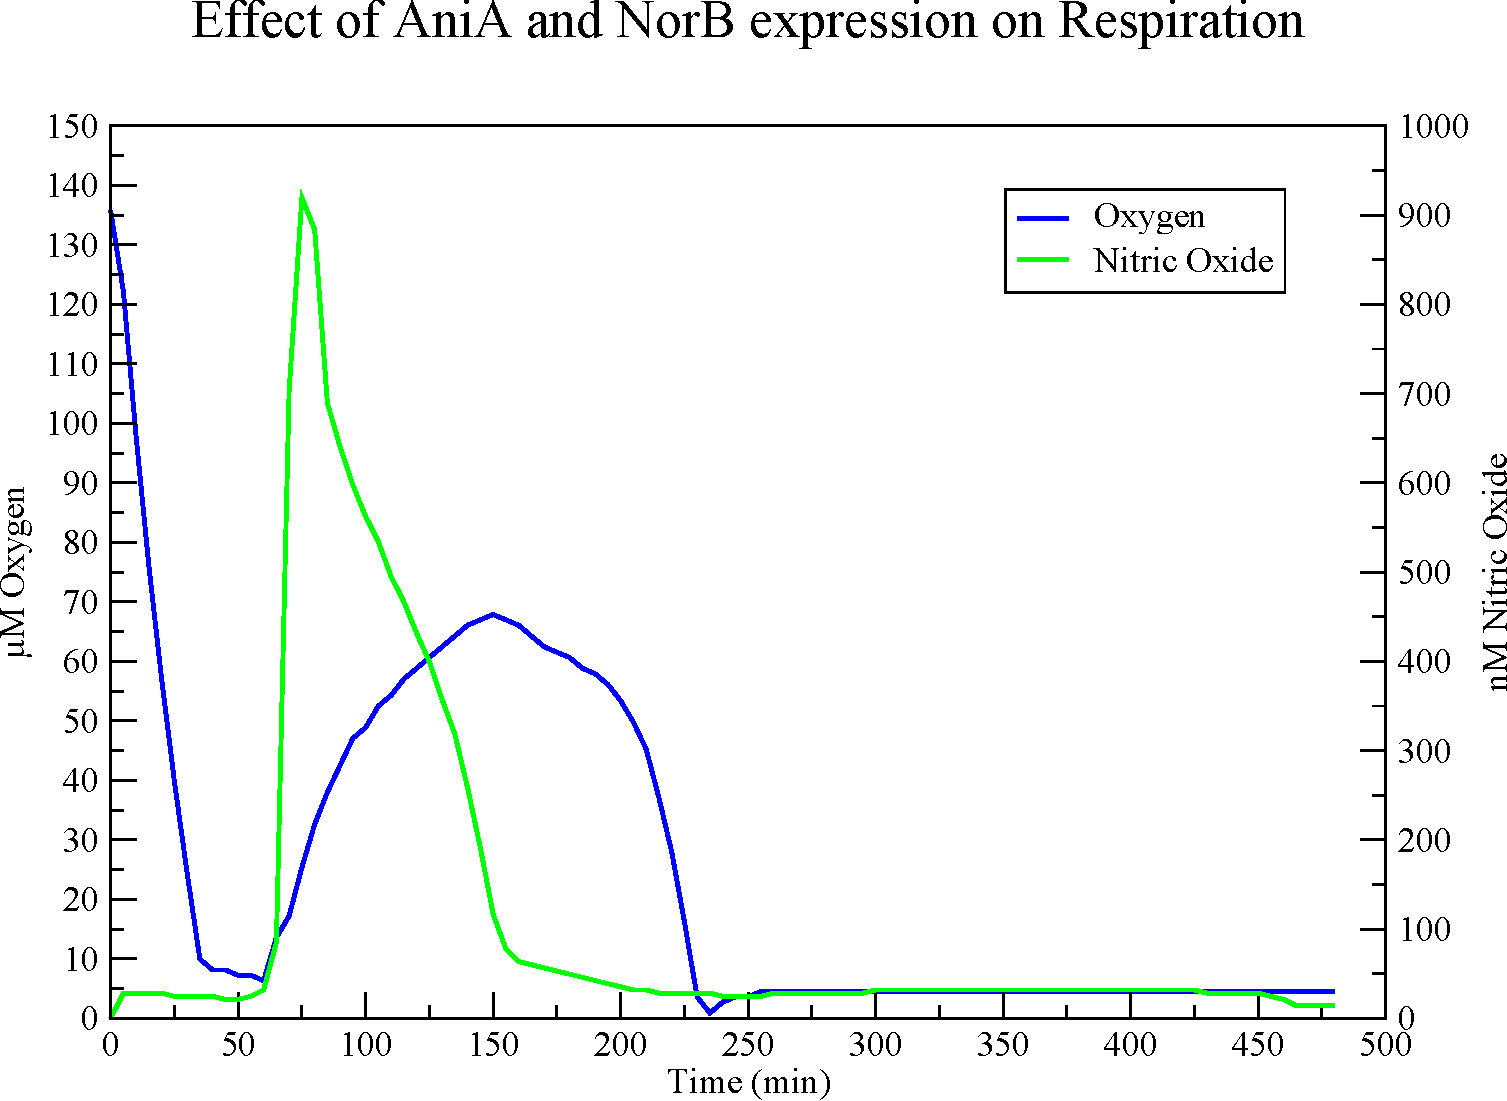
\includegraphics[height=10cm]{./08-expression/data/expression.pdf}
 % expression.pdf: 723x528 pixel, 72dpi, 25.51x18.63 cm, bb=0 0 723 528
 \caption[Effect of Expression of AniA and NorB]{{\bf Effect of Expression of AniA and NorB}. This figure shows an aerobically respiring culture in media with nitrite present. When oxygen is depleted, AniA and NorB begin to be expressed causing in increase and then decrease of NO. While NO is being reduced, Oxygen concentration slowly rises due to diffusion, and begins to be reduced once more when NO is depleted. Data from \citet{Rock2005}.
 \label{fig:expression}}
\end{figure}